%Notes by Harsh Mistry 
%Econ 301
%Based on Template From  https://www.cs.cmu.edu/~ggordon/10725-F12/template.tex

\documentclass[twoside]{article}
\setlength{\oddsidemargin}{0.25 in}
\setlength{\evensidemargin}{-0.25 in}
\setlength{\topmargin}{-0.6 in}
\setlength{\textwidth}{6.5 in}
\setlength{\textheight}{8.5 in}
\setlength{\headsep}{0.75 in}
\setlength{\parindent}{0 in}
\setlength{\parskip}{0.1 in}
\usepackage{amsmath,amsfonts,graphicx, color}
\newcounter{lecnum}
\renewcommand{\thepage}{\thelecnum-\arabic{page}}
\renewcommand{\thesection}{\thelecnum.\arabic{section}}
\renewcommand{\theequation}{\thelecnum.\arabic{equation}}
\renewcommand{\thefigure}{\thelecnum.\arabic{figure}}
\renewcommand{\thetable}{\thelecnum.\arabic{table}}
\newcommand{\lecture}[4]{
   \pagestyle{myheadings}
   \thispagestyle{plain}
   \newpage
   \setcounter{lecnum}{#1}
   \setcounter{page}{1}
   
   
%Info Box 
   \begin{center}
   \framebox{
      \vbox{\vspace{2mm}
    \hbox to 6.28in { {\bf Econ 301 - Microeconomic Theory 2
	\hfill Winter 2018} }
       \vspace{4mm}
       \hbox to 6.28in { {\Large \hfill Lecture #1: #2  \hfill} }
       \vspace{2mm}
       \hbox to 6.28in { {\it Lecturer: #3 \hfill Notes By: #4} }
      \vspace{2mm}}
   }
   \end{center}
   
   \markboth{Lecture #1: #2}{Lecture #1: #2}



 
}

\renewcommand{\cite}[1]{[#1]}
\def\beginrefs{\begin{list}%
        {[\arabic{equation}]}{\usecounter{equation}
         \setlength{\leftmargin}{2.0truecm}\setlength{\labelsep}{0.4truecm}%
         \setlength{\labelwidth}{1.6truecm}}}
\def\endrefs{\end{list}}
\def\bibentry#1{\item[\hbox{[#1]}]}

\newcommand{\fig}[3]{
			\vspace{#2}
			\begin{center}
			Figure \thelecnum.#1:~#3
			\end{center}
	}
	
	\graphicspath{ {images/} }

\newtheorem{theorem}{Theorem}[lecnum]
\newtheorem{lemma}[theorem]{Lemma}
\newtheorem{ex}[theorem]{Example}
\newtheorem{proposition}[theorem]{Proposition}
\newtheorem{claim}[theorem]{Claim}
\newtheorem{corollary}[theorem]{Corollary}
\newtheorem{definition}[theorem]{Definition}
\newenvironment{proof}{{\bf Proof:}}{\hfill\rule{2mm}{2mm}}
\newcommand\E{\mathbb{E}}


%Start of Document 
\begin{document}

\lecture{11}{February 12, 2018}{Jean Guillaume Forand}{Harsh Mistry}

\section{Competitive Equilibrium Continued}
\begin{ex} Say \(\omega^A = \left(\frac{1}{4}\right)\), \(\omega^B = \left(\frac{3}{4}, \frac{3}{4}\right)\) and \(u^A(x_1^A, x_2^A) = \ln x_1^A + x_2^A\) , \(u^B(x_1^B, x_2^B) = x_1^B + x_2^B \) 
\begin{center}
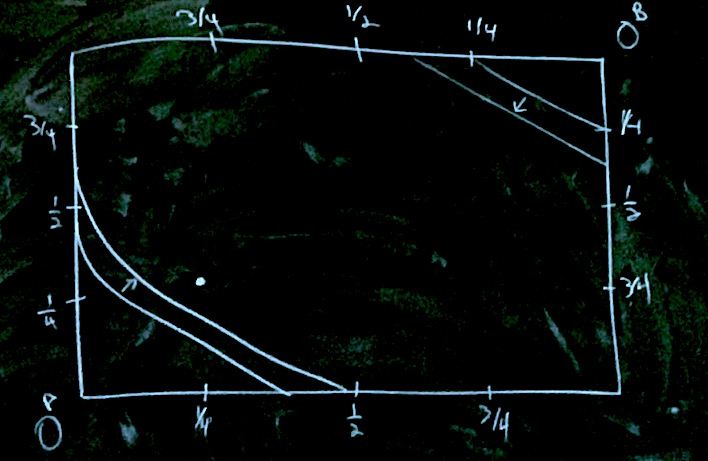
\includegraphics[scale=0.3]{16}
\end{center}
\begin{itemize}
\item Given prices \((p_1, p_2)\). UMP of consumer A. 
\[\max_{x_1, x_2 \geq 0} \ln x_1^A + x_2^B \hspace{0.2cm} \text{ s.t. } p_1x_1^A + p_2x_2^A \leq \frac{1}{4}p_1 + \frac{1}{4}p_2\]
\item Demand functions of A 
\[(x_1^A, (p\omega^A), x_2^A(p\omega^A)) = 
\begin{cases}
\left(\frac{p_1 + p_2}{4p_1},0 \right)& \hspace{0.2cm} \text{ if } \frac{p_1}{p_2} \leq 3 \\
\left(\frac{p_2}{p_1}, \frac{p_1 - 3p_1}{4p_2}\right) & \hspace{0.2cm} \text{ if } \frac{p_1}{p_2} > 3
\end{cases} \]
\item UMP of Consumer B 
\[\max_{x_1, x_2 \geq 0} x_1^B + x_2^B \hspace{0.2cm} \text{ s.t. } p_1x_1^A + p_2x_2^A \leq \frac{3}{4}p_1 + \frac{3}{4}p_2\]
\item Demand functions of B
\[(x_1^B, (p\omega^B), x_2^B(p\omega^B)) = 
\begin{cases}
\left(\frac{3p_1 + 3p_2}{4p_1},0 \right)& \hspace{0.2cm} \text{ if } \frac{p_1}{p_2} < 1 \\
\left(0, \frac{3p_1 + 3p_2}{4p_2}\right) & \hspace{0.2cm} \text{ if } \frac{p_1}{p_2} > 3
\end{cases} \]
\item Normalize \(p_1^* = 1\), find prices \((1, p_1^*)\) that clear one of the goods market 
\item Case 1:  Can we have \(\frac{1}{p_1^*} > 3\) ? (MC2) is not satisfied
\[\begin{aligned} x_2^A (p_1^* \omega^A) + x_2^A(p_1^*, \omega^B) & = \frac{1-3p_2^*}{4p_2^*} + \frac{3+3p_2^*}{3p_2^*}  = \frac{1}{p_2^*} \\
\end{aligned}\]
\item Case 2:  Can we have \(1 < \frac{1}{p_1^*} \leq 3\)? (MC2) is not satisfied
\[\begin{aligned} x_2\frac{1-3p_2^*}{4p_2^*} + \frac{3+3p_2^*}{3p_2^*}  = \frac{1}{p_2^*} ^A (p_1^* \omega^A) + x_2^A(p_1^*, \omega^B) & = \frac{3 + 3p_2^*}{4p_2^*}  = \frac{3}{4} + \frac{3}{4} (\frac{1}{p_2^*}) \\
& > \frac{3}{2} > 1 = \omega_2^A + \omega^B_2 \\
\end{aligned}\]
\item Case 3: Can we have \(\frac{1}{p_1^*} > 1\) ? (MC2) is not satisfied
\[\begin{aligned} x_2\frac{1-3p_2^*}{4p_2^*} + \frac{3+3p_2^*}{3p_2^*}  = \frac{1}{p_2^*} ^A (p_1^* \omega^A) + x_2^A(p_1^*, \omega^B) & = 0 < 1 = \omega^A_2 + \omega_2^B  
\end{aligned}\]
\item Case 4: Can we have \(\frac{1}{p_1^*} = 1\) ? (MC1) is satisfied
\[\begin{aligned} x_2\frac{1-3p_2^*}{4p_2^*} + \frac{3+3p_2^*}{3p_2^*}  = \frac{1}{p_2^*} ^A (p_1^* \omega^A) + x_2^A(p_1^*, \omega^B) & = \frac{1}{2} + x_1^B(p_1^* \omega^B) = 1\\
& \implies x_1^B (p^*_1 \omega^B) = \frac{1}{2}\\
& \implies \text{ Given budget constraint } x_2^B(p_1^* \omega^B) = 1
\end{aligned}\]
\item Prices (1,1) and allocations \((x_1^{A*}, x_2^{A*}) = \left(\frac{1}{2},0\right)\) and \((x_1^{B*}, x_2^{B*}) = \left(\frac{1}{2}, 1 \right)\) form a competitive equilibrium
\end{itemize}
\end{ex}

\begin{ex} Say \(\omega^A = (3, 1)\), \(\omega^B = (1, 2)\), \(u^A(x_1^A, x_2^A) = \min\{x_1^A, x_2^B\}\), and \(u^B (x_1^B, x_2^B) = \min \{x_1^B, x_2^B\} \)
\begin{center}
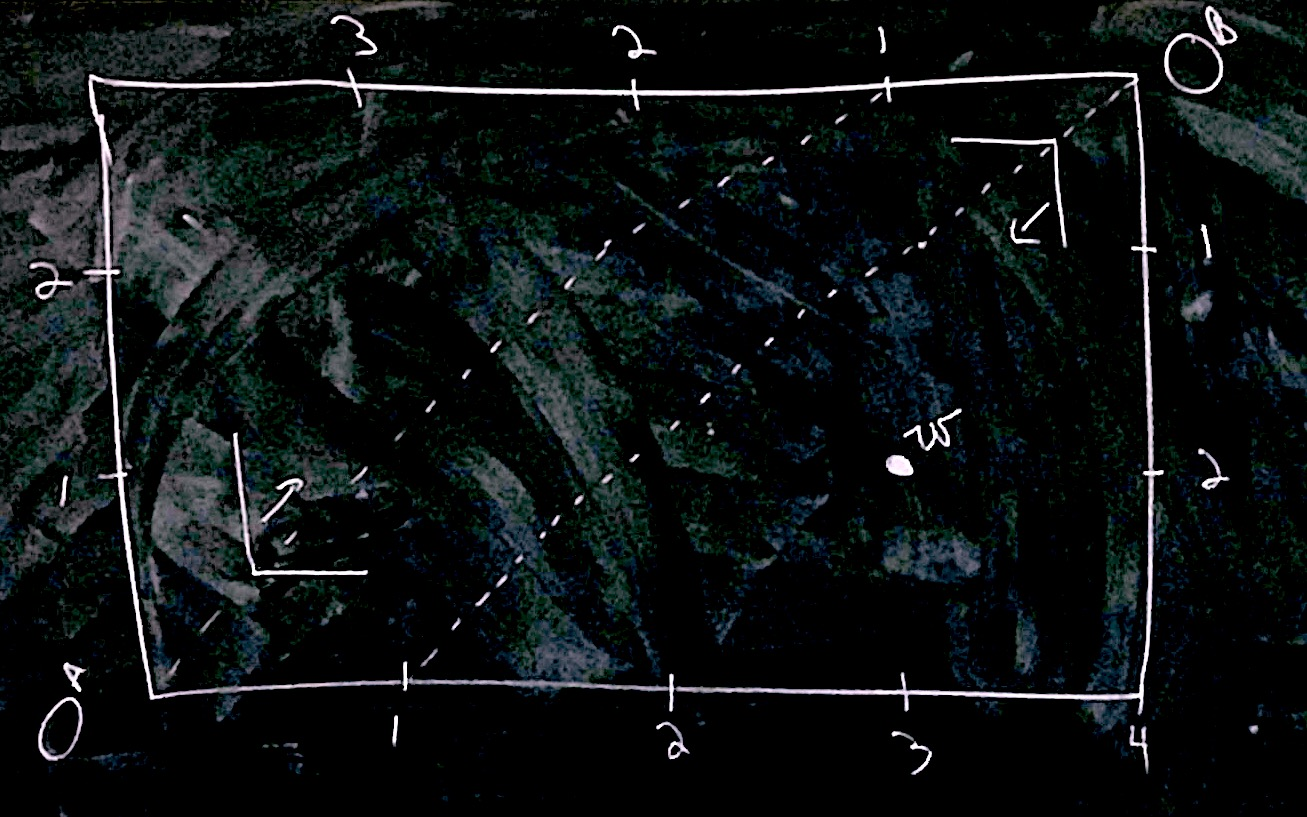
\includegraphics[scale=0.2]{17}
\end{center}
\begin{itemize}
\item Can we have \(p_1^*, p_2^* \neq 0\)? (MC1) fails 
\[\begin{aligned} x_1^A(p_1^*\omega^A) + x_1^B (p_1^* \omega^B) & = \frac{3p_1^* + p_2^*}{p_1^* + p_2^*} + \frac{p_1^* + 2p_2^*}{p_1^* + p_2^*} \\
 & = \frac{4p_1^* + 3p_2^*}{p_1^* + p_2^*} \\
 & = 3 + \frac{p_1^*}{p_1^* + p_2^* } < 4 \\
 & = \omega^B_1 + \omega^B_1
 \end{aligned}\]
\item Can we have \(p_1^* = 0\) ? 
\begin{itemize}
\item Demand functions for \(J = A, B\) : 
\[(x_1^J (p_1\omega^J), x_2^J(p_1 \omega^J)) = (\text{any } x_1^J \geq \omega^J_2 , \omega^J_2)\]
\end{itemize}
\(\implies\) Given any \(1 \leq x_1^{A*} \leq 2\), \(p^* = (0, 1) \) and allocations \(x_1^{A*} = (x^A, 1) \) and  \(x_{B*} = (4 - x^A_1 , 2) \) form a competitive equilibrium 
\begin{itemize}
\item Additional case : Can we have \(p_2^* =0 \)? No, (MC2) fails
\[\begin{aligned}x_2^A(p_1^*\omega^A) + x_2^B(p_1^*, \omega^A) & \geq \omega^A_1 + \omega_1^B \\ & = 4 \\ & > 3 = \omega_2^A + \omega^B_2 
\end{aligned}\]
\end{itemize}
\end{itemize}
\end{ex}
\end{document}





